\documentclass[reprint,english,notitlepage,nofootinbib]{revtex4-1}  %

\usepackage{silence}
\WarningFilter{revtex4-1}{Repair the float}
\usepackage[sorting=none, bibstyle=ieee]{biblatex}
\addbibresource{references.bib}
\usepackage[utf8]{inputenc}
\usepackage[english]{babel}
\usepackage{physics,amssymb} 
\usepackage{graphicx}        
\usepackage{xcolor}          
\usepackage{hyperref}        
\usepackage{tikz, pgfplots}
\usepackage{listofitems}
\usepackage{listings}
\usepackage{csquotes}
%\usepackage{subfigure}  
\usepackage{here}
\usepackage{fancyvrb}
\usepackage{fontawesome}
\usepackage{fontspec}
\usepackage{algorithm}
\usepackage{algorithmic}
\usepackage{subcaption}
%\bibliographystyle{plain}
\hypersetup{ % this is just my personal choice, feel free to change things
    colorlinks,
    linkcolor={red!50!black},
    citecolor={blue!50!black},
    urlcolor={blue!80!black}}

%% Defines the style of the programming listing
%% This is actually my personal template, go ahead and change stuff if you want
\lstset{ %
	inputpath=,
	backgroundcolor=\color{white!88!black},
	basicstyle={\ttfamily\scriptsize},
	commentstyle=\color{magenta},
	language=Python,
	morekeywords={True,False},
	tabsize=4,
	stringstyle=\color{green!55!black},
	frame=single,
	keywordstyle=\color{blue},
	showstringspaces=false,
	columns=fullflexible,
	keepspaces=true}

 %% TiKz stuff
\usetikzlibrary{positioning, chains}
\colorlet{myred}{red!80!black}
\colorlet{myblue}{blue!80!black}
\colorlet{mygreen}{green!60!black}
\colorlet{myorange}{orange!70!red!60!black}
\colorlet{mydarkred}{red!30!black}
\colorlet{mydarkblue}{blue!40!black}
\colorlet{mydarkgreen}{green!30!black}

\definecolor{mako1}{HTML}{38aaac}
\definecolor{mako2}{HTML}{357ba3}
\definecolor{mako3}{HTML}{40498e}

% STYLES
\tikzset{
  >=latex, % for default LaTeX arrow head
  node/.style={thick,circle,draw=mako1,minimum size=22,inner sep=0.5,outer sep=0.6},
  node in/.style={node,black,draw=mako1!30!black,fill=mako1!40},
  node hidden/.style={node,black,draw=mako2!30!black,fill=mako2!40},
  node out/.style={node,black,draw=mako3!30!black,fill=mako3!40},
  connect/.style={->,thick,mako3!40!black}, %,line cap=round
  connect arrow/.style={-{Latex[length=4,width=3.5]},thick,mako3!40!black,shorten <=0.5,shorten >=1},
  node 1/.style={node in}, % node styles, numbered for easy mapping with \nstyle
  node 2/.style={node hidden},
  node 3/.style={node out}
}
\def\nstyle{int(\lay<\Nnodlen?min(2,\lay):3)}


\begin{document}

%==========================================================
%------------------ Project content -----------------------
%==========================================================

%------------------ Title ---------------------------------
\title{TITLE}
\author{Even Sletteng Garvang, Ellen-Beate Tysvær, Janita Ovidie Sandtrøen Willumsen \\ \faGithub \, \url{https://github.com/evengar/FYS-STK4155-Project3}}        
\date{\today}
\noaffiliation

\begin{abstract}
Plankton bla bla
\end{abstract}
\maketitle

%------------------ Body ----------------------------------
%\mainmatter
\section{Introduction}\label{sec:introduction}

The marine pelagic environment, that is, the free water masses in the ocean, is the largest ecosystem on the planet (REF). The biomass in the pelagic is dominated by plankton (REF), which by definition are organisms that can not move against the current. Primary producers in the pelagic, phytoplankton, produce 50 \% of earth's oxygen, and are at the base of the food chain (REF). Small zooplankton, such as copepods, consume the phytoplankton and are food for higher consumers, like larvae of commercially important fish species.

To understand the ecosystem dynamics in the pelagic it is important to have good estimates of biomass and species composition of the plankton. However, traditional enumeration of plankton is a time-consuming process that requires extensive taxonomic expertise to differentiate the vast amount of plankton species. Recently, automated plankton imagers have become widespread to combat this issue. Instruments like the PlanktoScope \cite{pollina2022:planktoscope} can quantitatively image both phytoplankton and zooplankton. These instruments still require taxonomic knowledge to manually differentiate species, representing a major hurdle in high-throughput plankton quantification.

In recent years, as machine learning (ML) methods have become more advanced, the models have become more difficult to interpret. Decision trees are widely used as a supervised ML method because of their simple yet powerful nature, which makes them useful as baseline models when exploring more complex models. They can be utilized for both classification and regression problems, are non-parametric, and can provide insight by organizing the data in a tree structure. Decision trees can be improved through boosting methods, for example AdaBoost \cite{zou2009}.

Since their introduction in 1989 \cite{lecun1989}, convolutional neural networks (CNNs) have been widely used for image analysis, and successfully applied in, e.g., facial recognition, handwritten digit recognition, and medical imaging contexts \cite{li2022}. In contrast to the widespread fully-connected feed-forward neural networks (FCNNs), the architecture of CNNs are tailored for, e.g., image recognition tasks (see methods), and perform better in these contexts. 

Classification with both CNNs and decision trees are examples of supervised machine learning algorithms, where training of the network or tree depends on having pre-labeled data, that the algorithm then compares its output with. Unsupervised machine learning is an alternative to this, where the input data is sorted into clusters or groups without using pre-assigned labels \cite{olaode2014}. Unsupervised learning has been successfully applied to categorize biological data, including plankton \cite{pastore2023}.

In 2017, a novel architecture for deep learning was introduced with the infamous article "Attention is all you need" \cite{attention}. This architecture is today known as the transformer, and it formed the basis for the current AI wave which includes major names such as ChatGPT, Dal-E and AlphaFold 2. The transformer architecture was originally thought to replace recurrent neural networks (RNN) as the model of choice for translation of text. The model had several novel ways to train a network,
but the main focus was a new mechanism called "self-attention" (methods).

Only three years after the first transformer architecture was introduced, the article "An Image is Worth 16x16 Words: Transformers for Image Recognition at Scale" \cite{first_vit} introduced the first functional transformer trained on images, and it was baptized as a Vision Transformer (ViT). The authors demonstrate how a ViT outperforms classical deep learning methods such as CNN. 

A model named "self-distillation with no labels" (DINO) was introduced by Facebook (now Meta) shortly after the original ViT was proposed \cite{dino1}, as a self-supervised computer vision method inspired by the "Bootstrap your own latent"-method of self-supervision \cite{byol}. The authors found that DINO works exceptionally well with ViT architechtures, and their model achieved 80.1\% top-1 on ImageNet in linear evaluation. We use the second iteration of DINO, DINO v2 \cite{dino2} in the current study.

Here we apply several ML models to classify plankton image data from two different imagers. First, we apply a decision tree and AdaBoost to pre-extracted features from the data to investigate which classical features (length, width, opacity etc.) are most important for classification. Then, we train a CNN on the images and assess classification performance. Finally, we apply DINO v2 to extract features from the images, and use these features both directly for clustering, and as input for decision trees with and without AdaBoost. We compare the performance of all models, and discuss their applicability in plankton classification. We also discuss the potential of using unsupervised learning for pre-sorting large amounts of plankton data to streamline processing.
\section{Methods}\label{sec:methods}

% =========================================================================
%
% EB writes here - this is method but parts of it can also be included in introduction.

\subsection{Vision Transformers} %\label{ssec:vit}
In 2017, a novel architecture for deep learning was introduced with the infamous article 
"Attention is all you need" \cite{attention}. This architecture is today known as the 
transformer, and it formed the basis for the current AI wave which includes major 
names such as ChatGPT, Dal-E and AlphaFold 2.

The transformer architecture was originally thought to replace recurrent neural networks (RNN)
as the model of choice for translation of text. The model had several novel ways to train a network,
but the main focus was on the attention mechanism. We will not go into detail on the attention
mechanism here, but it is worth a mention that this concept introduced in 2014 \cite{first_attention}
provides the network with more context for each data point that it tries to predict, which is one
of the aspects that made transformers superior in predicting and later producing full sentences. 

Only three years after the first transformer architecture was introduces, the article 
"An Image is Worth 16x16 Words: Transformers for Image Recognition at Scale" \cite{first_vit}
introduced the first functional transformer trained on images, and it was baptized as a Vision
Transformer (or ViT for short). The authors demonstrate how a ViT outperforms classical 
deep learning methods such as convoultional neural networks (CNN). 

A ViT splits an image into even sized, non-overlapping patches, which are then linearly embedded
as token representations. These tokens are then fed into the regular transformer architecture with 
their positional embeddings. The previously mentioned attention mechanism is then used during training
so that the model considered spatial relationships within and between patches. 

The authors of this 
report will not pretend to understand the ViT completely, but we provide the reader with all sources
to fully comprehend this novel architecture, and present the original layout of a ViT in Figure \ref{fig:ViT}

\begin{figure}[H]
    \centering
    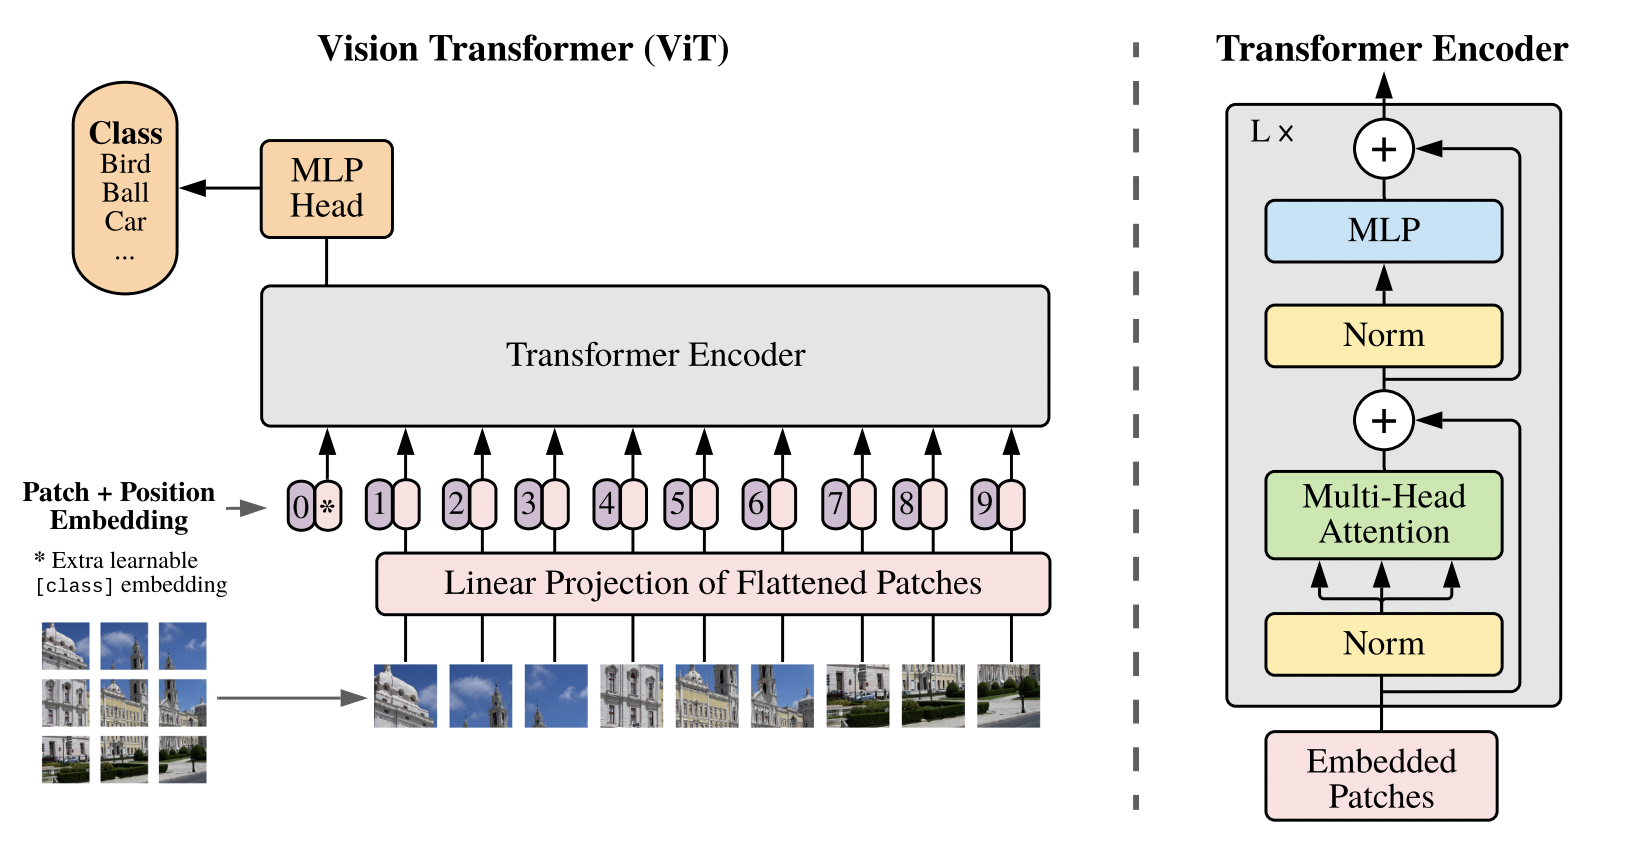
\includegraphics[width=1.1\linewidth]{examples/tests_eb/figs/vit.png}
    \caption{Vision Transformer layout as presented from it's original paper by Dosovitskiy et. al \cite{first_vit}}
    \label{fig:ViT}
\end{figure}

\subsubsection{Self-\textbf{di}stillation with \textbf{no} labels (Meta's \textbf{DINO})} \label{sssec:dino}
The first DINO was introduced by Facebook (now Meta) shortly after the original ViT was proposed \cite{dino1}, as a self-supervised computer vision method inspired by the "Bootstrap your own latent"-method of self-supervision \cite{byol}. The authors found that DINO works exceptionally well with ViT architechtures, and their model achieved 80.1\% top-1 on ImageNet in linear evaluation.  

The self-\textbf{di}stillation aspect refers to a teacher-student interaction, where a teacher model looks into global augmented crops of an image and the student model looks into both smaller (local), augmented crops and global, augmented crops of the same image. The goal is that both the student and the teacher gives us the same feature representation of the different crops, essentially teaching the model that minor deviations in size and color should still fall into the same representation. A simple figure from the original article is shown in Figure \ref{fig:dino}.

\begin{figure}[H]
    \centering
    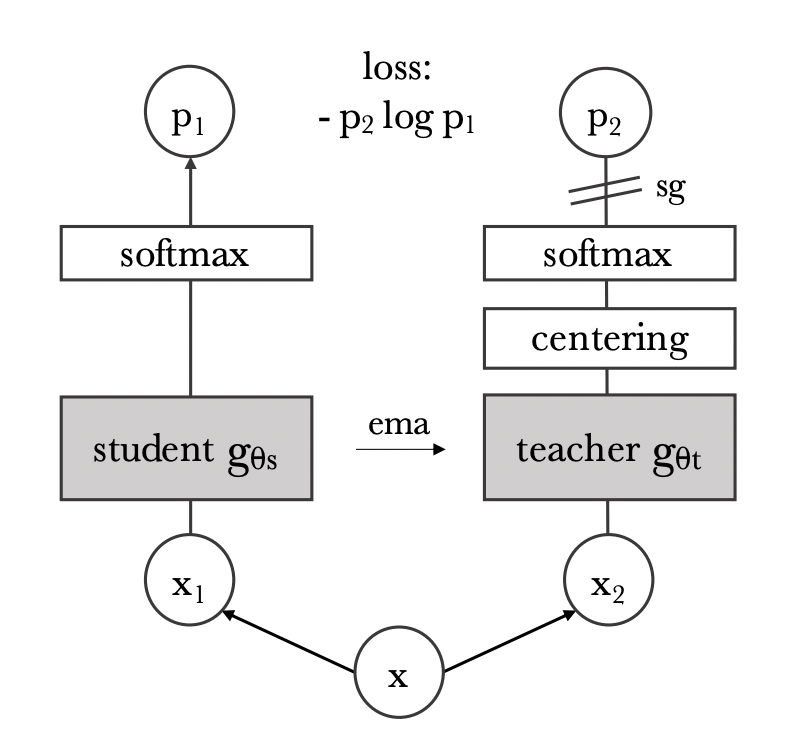
\includegraphics[width=0.7\linewidth]{examples/tests_eb/figs/dino.png}
    \caption{Student-Teacher interactions as presented in original DINO article \cite{dino1}.}
    \label{fig:dino}
\end{figure}

We will not give a full explanation of the DINO functionality, but it is important to note that it is self-supervised and has shown exceptional performance on extracting a set of features to represent an image. 

This performance has since increased with Meta's newest release of the updated \textbf{DINOv2} \cite{dino2} from january 2024, which they offer as an open source, pre-trained ViT model of 1B parameters. The model produces a set of visual features and has been trained on LVD-142M, meaning 142 million images. The authors themselves make the claim that the newest DINOv2 does not require any fine tuning, and we've therefore chosen to go for their reccomended approach. 


%
% =========================================================================

% =========================================================================
%
% Janita writes here
%
% =========================================================================

% =========================================================================
%
% Even writes here
%
% =========================================================================
\section{Results}\label{sec:results}

% ==================================================================
%
% EB writes here
%

\begin{figure}[H]
    \centering
    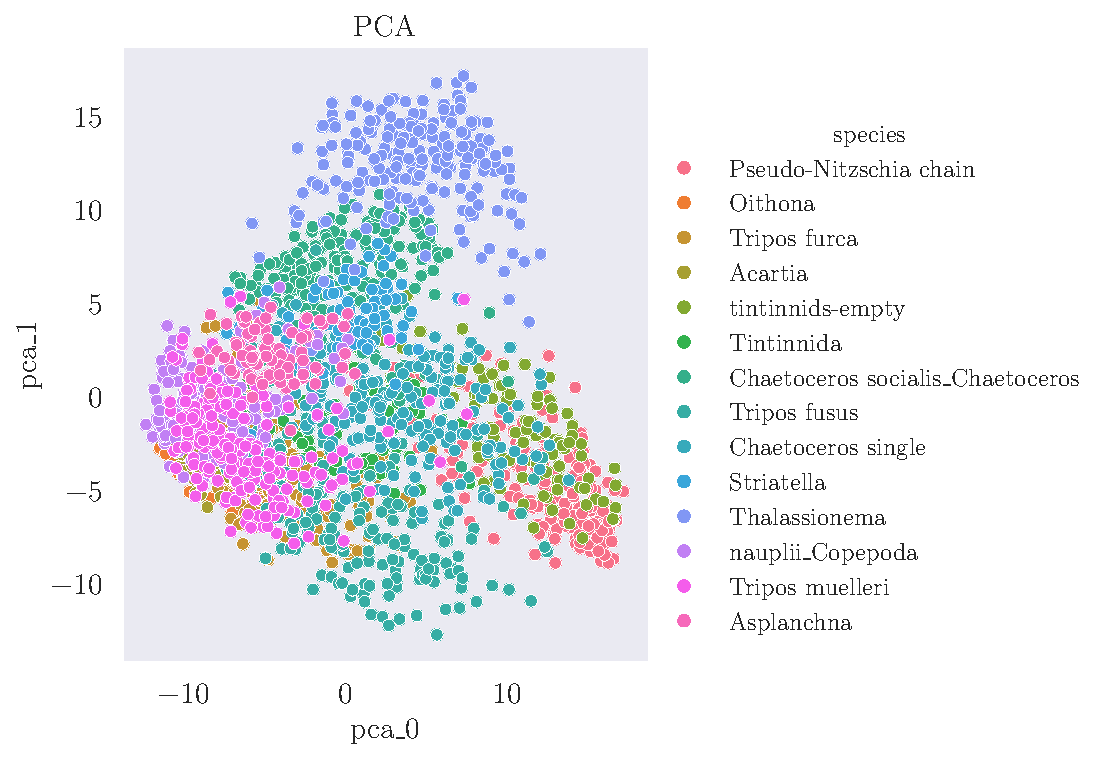
\includegraphics[width=1.1\linewidth]{examples/tests_eb/figs/pca0_pca1.pdf}
    \caption{The two first principal components out of 70 plotted against each other. Already here we can see some weak signs of clusters}
    \label{fig:pca0pca1}
\end{figure}

\begin{figure}[H]
    \centering
    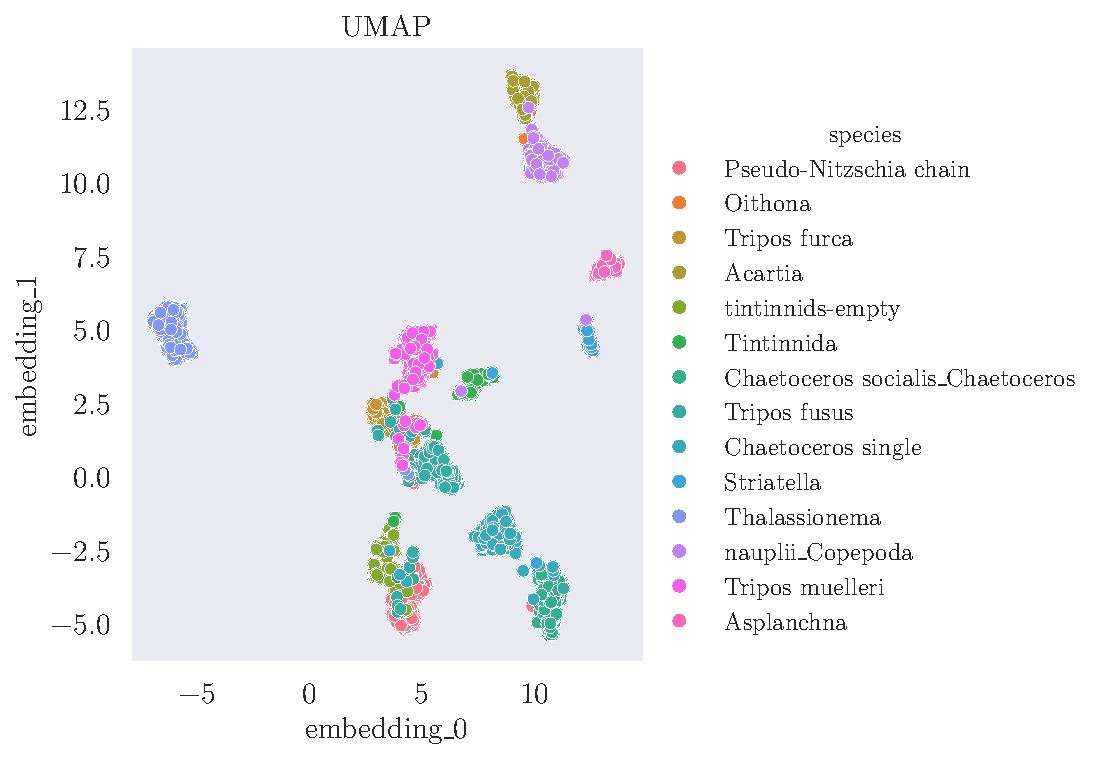
\includegraphics[width=1.1\linewidth]{examples/tests_eb/figs/umap.pdf}
    \caption{A UMAP plot to explore non-linear relations in our data (TODO - read up on UMAP). Here we can clearly see how our extracted features cluster together, yet we still do not have 14 distinct clusters.}
    \label{fig:enter-label}
\end{figure}

% ==================================================================
\section{Conclusion}\label{sec:conclusion}
a
\newpage

 
%------------------ Bibliography --------------------------

\onecolumngrid
\newpage 
% \nocite{*}
\printbibliography

%------------------ Appendix ------------------------------
\newpage
\twocolumngrid
\appendix
\section{Apepndix}
\begin{figure}[H]
    \centering
    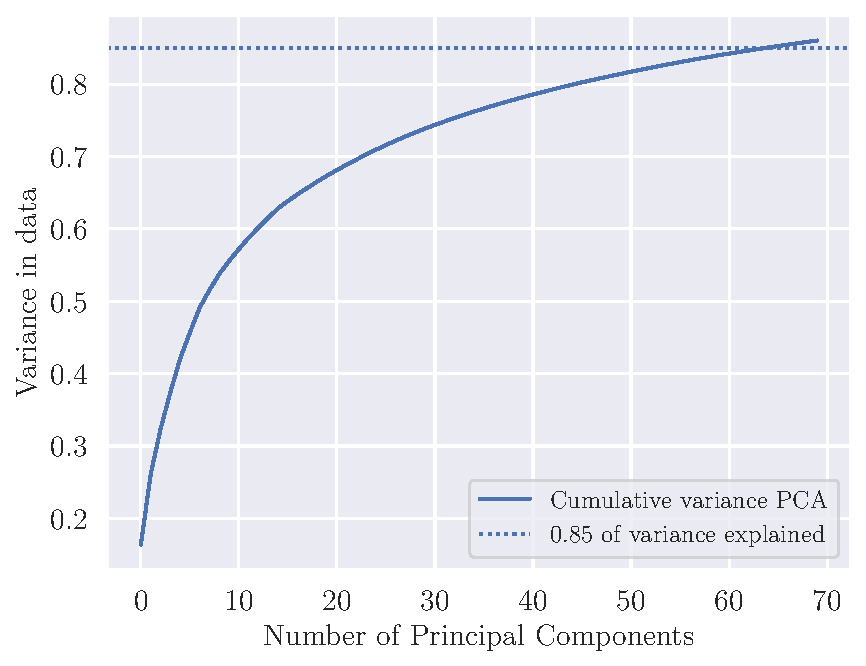
\includegraphics[width=0.9\linewidth]{examples/tests_eb/figs/cumsum_pca.pdf}
    \caption{A plot of the cumulative variance for each principle component included in our new, dimensionality reduced features. We concluded that 70 features was sufficient to capture just above 85 percent of the variance in our data.}
    \label{fig:cumsumpca}
\end{figure}

\begin{figure}[H]
    \centering
    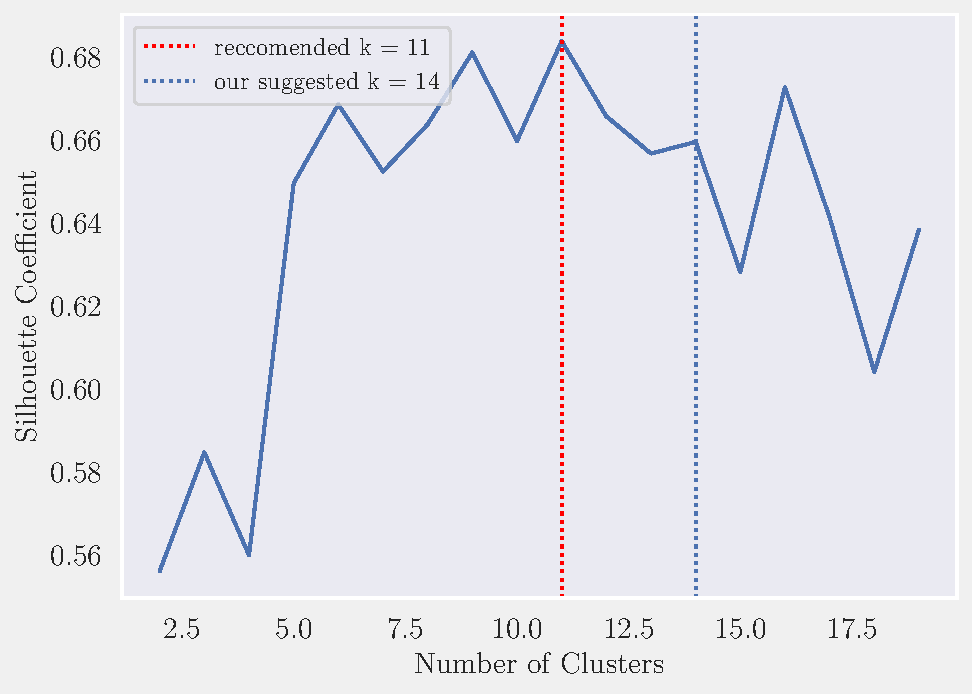
\includegraphics[width=0.9\linewidth]{examples/tests_eb/figs/kmean_sil.pdf}
    \caption{A plot of the silhouette scores for each KMean tested on UMAP data.}
    \label{fig_cumsumpca}
\end{figure}


\begin{figure}[H]
    \centering
    \begin{subfigure}[b]{1\linewidth}
        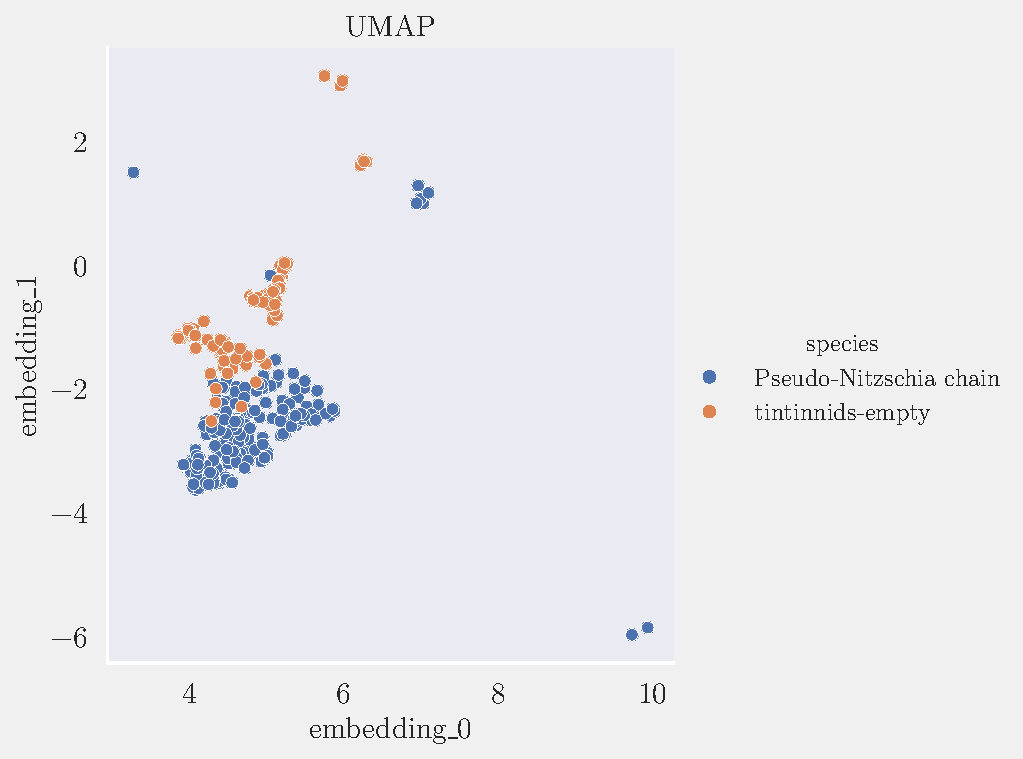
\includegraphics[width=\linewidth]{examples/tests_eb/figs/umap_on_two_species.pdf}
        \caption{First we isolated the already produced embeddings for the two species. Already her we can see that they form clysters according to their species.}
    \end{subfigure}
    
    \vspace{1em}
    
    \begin{subfigure}[b]{1\linewidth}
        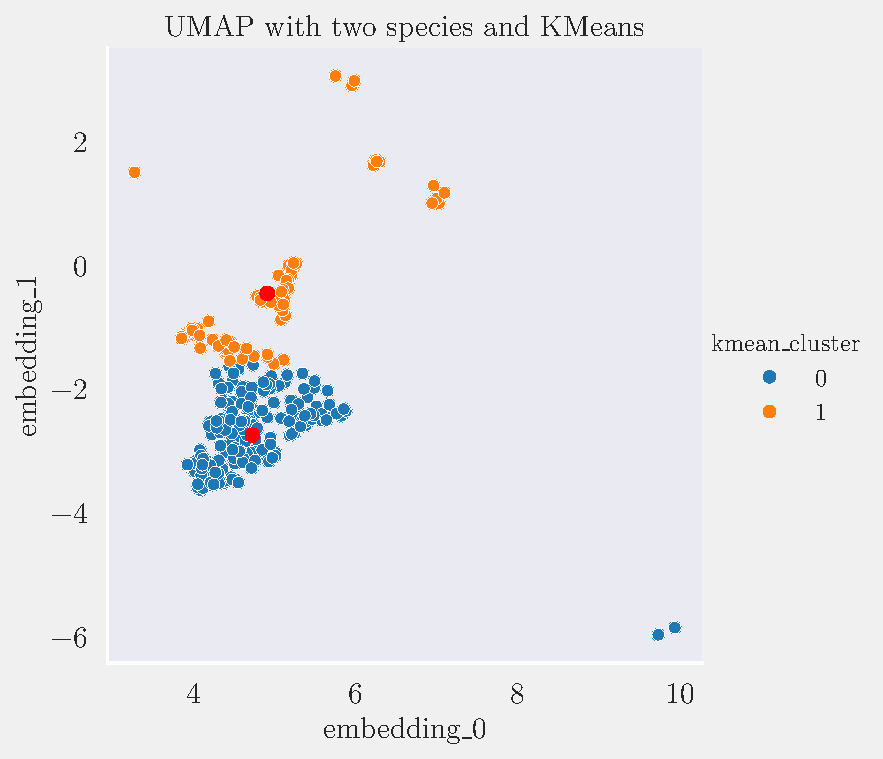
\includegraphics[width=\linewidth]{examples/tests_eb/figs/kmeans_cluster_umap_on_two_species.pdf}
        \caption{We performed a KMeans clustering with two clusters to find which images (or species) would cluster together in the embedding space. Red dots are kmer centroids.}
    \end{subfigure}
    \caption{The process of finding the images that misclusteded in Figure \ref{fig:misclusters} explained. We display images of Pseudo N that were placed in cluster 1, and the opposite for Tintinnids-e.}
    \label{fig:misclustering_process}
\end{figure}


%------------------ Structure -----------------------------
% \tableofcontents 

%==========================================================
%------------------ End of project content ----------------
%==========================================================
\end{document}